

We conducted several experiments for each of the tasks described in Chapter \ref{chap:contributions}. Each experiment is composed of a training phase and a evaluation phase.

\begin{itemize}
\item Training phase: In this phase the agent is actually learning by sampling data from the simulation server to actively update the parameters of the policy and value-functions, represented as neural networks.

\item Evaluation phase: After the training phase, we freeze all the parameters and eliminate the exploration gaussian noise, turning the policy deterministic. Also, since we trained using RSI, for evaluation we initialize the state in a constant instant. Finally, we assess the training performance by the metrics described in section \ref{sec:metrics}.
\end{itemize}

We trained each task using the Proximal Policy Optimization (PPO) algorithm. After the learning phase is completed, we compare the final obtained movement with the classical ZMP kick, in order to evaluate the mimic performance in imitating the joints commands and also the goal performance in reaching the desired ball final position.

As described in section \ref{sec:devcloud}, the training phases for all experiments were conducted in the Intel AI DevCloud.

\section{Supervised Kick Learning}

In the Supervised Kick Learning task, we ran training using Adam optimization \cite{adam}, applying 5 consecutive optimization cycles with 5000 epochs each one and decreasing the learning rate linearly, applying $0.001$, $0.0008$, $0.0006$, $0.0004$, $0.0002$ respectively for each cycle. The loss function used was the Mean Squared Error.

The other hyperparameters used follow the standard values found in the Literature, also presented in Table \ref{tab:SL}.

\begin{table}[ht]
    \begin{tabular}{|l|l|}
    \hline
    Hyperparameter            & Value    \\ \hline
    $\beta_1$ 	              & $0.9$ \\
    $\beta_2$                  & $0.999$     \\
    $\epsilon$                & $10^{-8}$     \\
    \hline
    \end{tabular}
\centering
\caption{Hyperparameters used for the Supervised Kick Learning.}
\label{tab:SL}
\end{table}

Figure \ref{fig:SL_MAE} shows the Mean Absolute Error for the first training cycle, and we can easily verify the efficiency for the training phase.

In the evaluation phase, we ran an agent using the obtained NN as the policy, and compared the joints commanded positions with the ZMP kick reference movement. Figure \ref{fig:SL_cmd_pos} shows the corresponding data for the right knee pitch joint.

\begin{figure}[H]
    \centering
    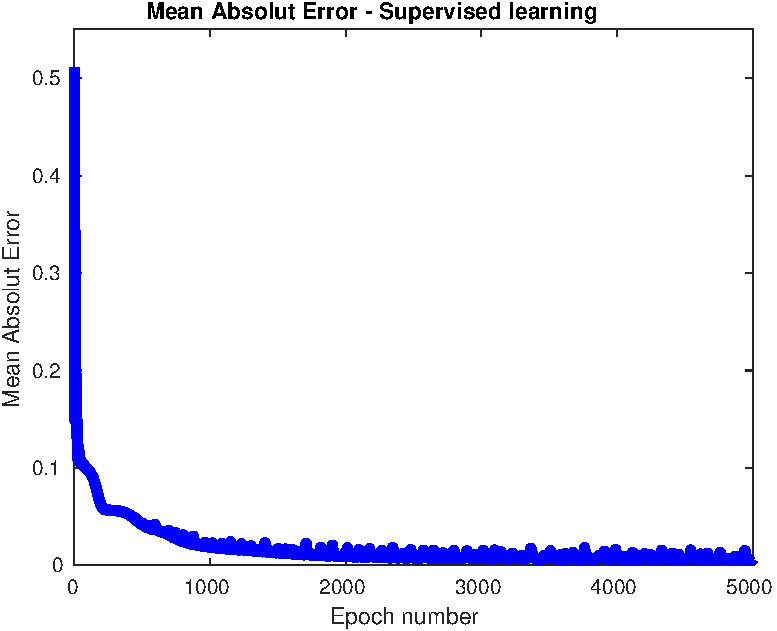
\includegraphics[width=0.6\textwidth]{Chapter7/plots/plot_MAE_supervised.pdf} 
    \caption{Mean Absolute Error - SL.}
    \label{fig:SL_MAE}
\end{figure}

\begin{figure}[H]
    \centering
    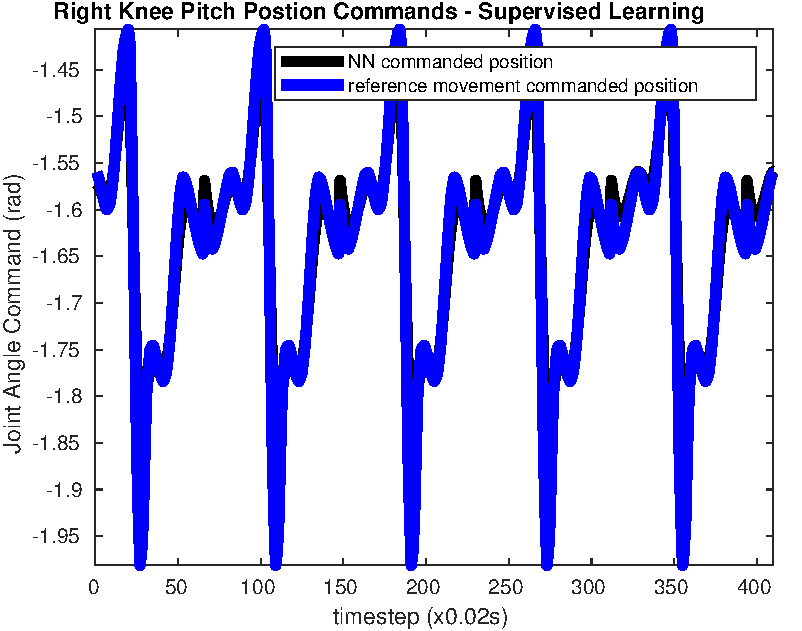
\includegraphics[width=0.6\textwidth]{Chapter7/plots/plot_joints_pos_superv.pdf} 
    \caption{Commanded Position for the Right Knee Pitch Joint - SL.}
    \label{fig:SL_cmd_pos}
\end{figure}

\section{Pure Mimic Learning}

In the Pure Mimic Learning experiment, we ran PPO with 1 simulated agent using  $2 \times 10^6$ total samples. The hyperparameters used are presented in Table \ref{tab:ppo_pure_mimic}.

The key adaptations which made possible to learning this task were: increasing the NN size, since smaller networks showed to be unsuccessful in mapping all the movement details; and restricting the episode length to include only the phases with actual swinging foot, i.e, only the phases B, C and D of the ZMP kick described in Section \ref{sec:ZMPkick}, which correspond to more subtle joints movements and with bigger influence in the ball's final position.

\begin{table}[ht]
    \begin{tabular}{|l|l|}
    \hline
    Hyperparameter            & Value    \\ \hline
    Adam stepsize             & $5 \times 10^{-5}$ \\
    Num. epochs               & $10$     \\
    Minibatch size            & $256$     \\
    GAE parameter ($\lambda$) & $0.95$   \\
    Discount ($\gamma$)		   & $0.99$	  \\
    Timesteps per batch       & $2048$   \\ \hline
    \end{tabular}
\centering
\caption{PPO hyperparameters used for Pure Mimic Learning.}
\label{tab:ppo_pure_mimic}
\end{table}

Figure \ref{fig:RL_mimic_reward} shows the total reward during the training phase, by its monotonic increasing we can see a clear success for this phase.

In the evaluation phase, we ran an agent using the obtained policy and compared joints positions commands. Figure \ref{fig:RL_cmd_pos} shows these commands for the Right Knee Pitch joint, comparing the mimic behavior with the ZMP kick reference movement. We can notice that that the NN commanded position contains a noise, corresponding to the gaussian exploration noise in the policy.

At the end, the agent was capable of kicking the ball towards a final distance very close to the one performed by the ZMP kick, as can be seen in Table \ref{tab:ppo_pure_mimic_stat}.

\begin{table}[ht]
    \begin{tabular}{|l|l|l|}
    \hline
      &     ZMP Kick          & Pure Mimic Behavior  \\ \hline
    Mean             &    $1.22$       &   $1.2151$       \\
    Std              &    $0.0629$     &   $0.0489$       \\ \hline
    \end{tabular}
\centering
\caption{Pure Mimic Results Statistics}
\label{tab:ppo_pure_mimic_stat}
\end{table}


\begin{figure}[H]
    \centering
    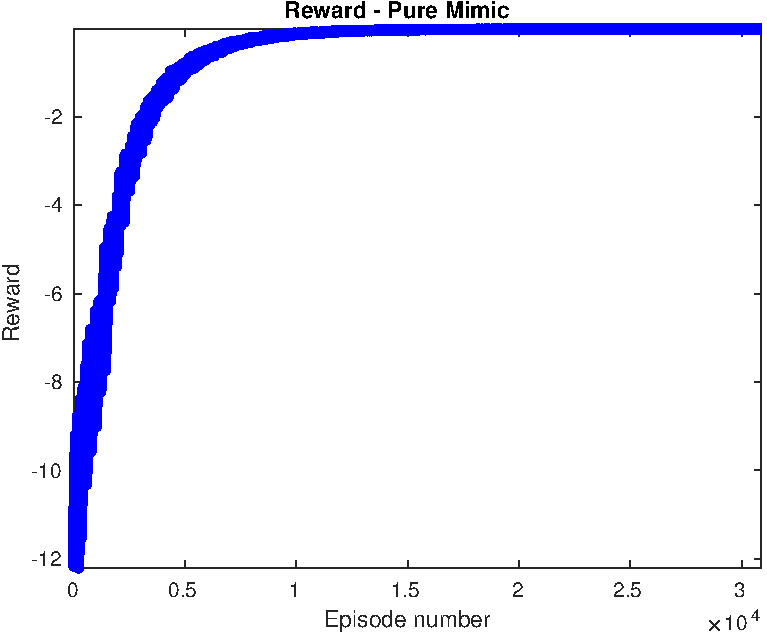
\includegraphics[width=0.6\textwidth]{Chapter7/plots/plot_reward_mimic.pdf} 
    \caption{Reward signal during training for the Pure Mimic task.}
    \label{fig:RL_mimic_reward}
\end{figure}

\begin{figure}[H]
    \centering
    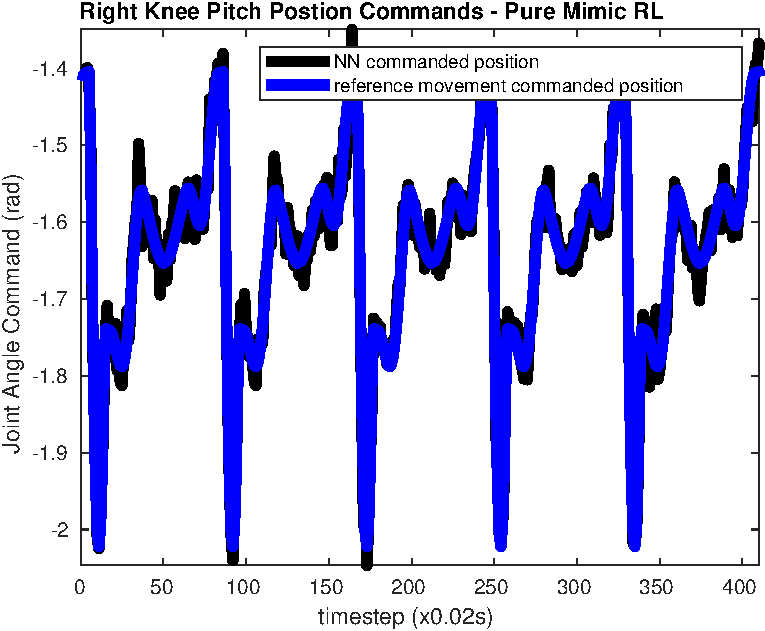
\includegraphics[width=0.6\textwidth]{Chapter7/plots/plot_joints_pos_mimic.pdf} 
    \caption{Commanded Position for the Right Knee Pitch Joint - mimic RL.}
    \label{fig:RL_cmd_pos}
\end{figure}

\section{Farthest Final Distance Learning}
\label{sec:far_kick_results}

In the Farthest Final Distance Learning experiment, we ran PPO with 20 simulated agents using $10^8$ total samples. The hyperparameters used are presented in Table \ref{tab:ppo_far_kick}.

\begin{table}[ht]
    \begin{tabular}{|l|l|}
    \hline
    Hyperparameter            & Value    \\  \hline
    Adam stepsize             & $10^{-5}$ \\
    Num. epochs               & $10$     \\
    Minibatch size            & $2048$     \\
    GAE parameter ($\lambda$) & $0.95$   \\
    Discount ($\gamma$)       & $0.9999$ \\
    Timesteps per batch       & $4096$   \\ \hline
    \end{tabular}
\centering
\caption{PPO hyperparameters used for the Farthest Final Distance Learning.}
\label{tab:ppo_far_kick}
\end{table}

The key adaptations which made possible to learn this task were: Performing the Random State initialization (RSI), described in the Deep Mimic Section \ref{sec:deep_mimic}; increasing the discount factor ($\gamma$); increasing the minibatch size; and performing very long trainings.

Since the greatest fraction of the goal reward is only received at the end of the episode, because the agent finishes the movement before the ball stops, the reward function is still quite sparse. Increasing the $\gamma$ and performing the random state initialization helped to deal with this limitation, making possible to propagate the reward signal into more initial states.

Increasing the minibatch size was useful to deal with the big noise in ball's terminal positions during training. Small variations given by the exploration noise in the joints' commands can result in big differences observed for the ball position. Increasing the batch size and running for multiple agents made possible to reach a more reliable gradient estimate.

Performing long trainings was essential, since the agent takes some time to actually start to learn, as can be seen in the reward signal in Figure \ref{fig:RL_far_kick}. This usually happens because the agent needs to adapt the value function, pre-trained for the Pure Mimic task, to the new reward distribution.

\begin{figure}[H]
    \centering
    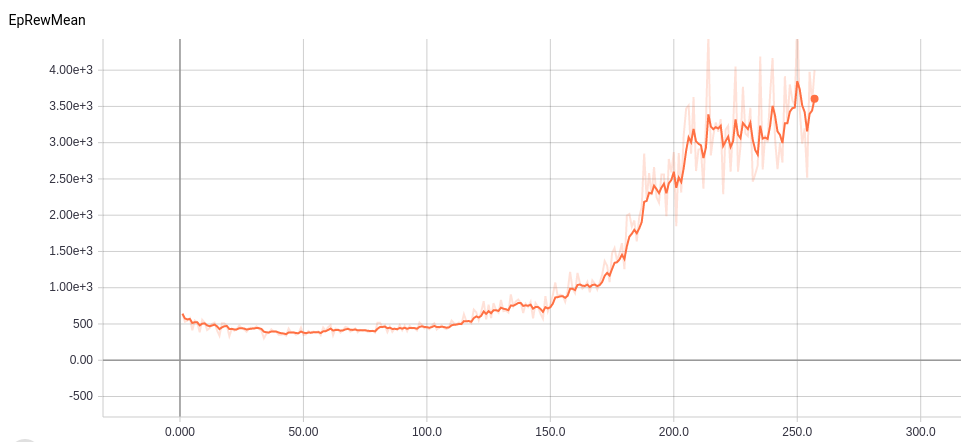
\includegraphics[width=0.8\textwidth]{Chapter7/figures/rew_mean_far_kick.png} 
    \caption{Reward signal during training for the Farthest Kick task.}
    \label{fig:RL_far_kick}
\end{figure}

Finally, we can see the success in the training phase by the episode average reward in Figure \ref{fig:RL_far_kick}. Besides, we plotted the final ball positions along this phase in Figure \ref{fig:RL_far_kick_pos_train}. We can see an overall increasing in the final positions, followed also by an increasing in its noise, which is mostly due to the RSI.

\begin{figure}[H]
    \centering
    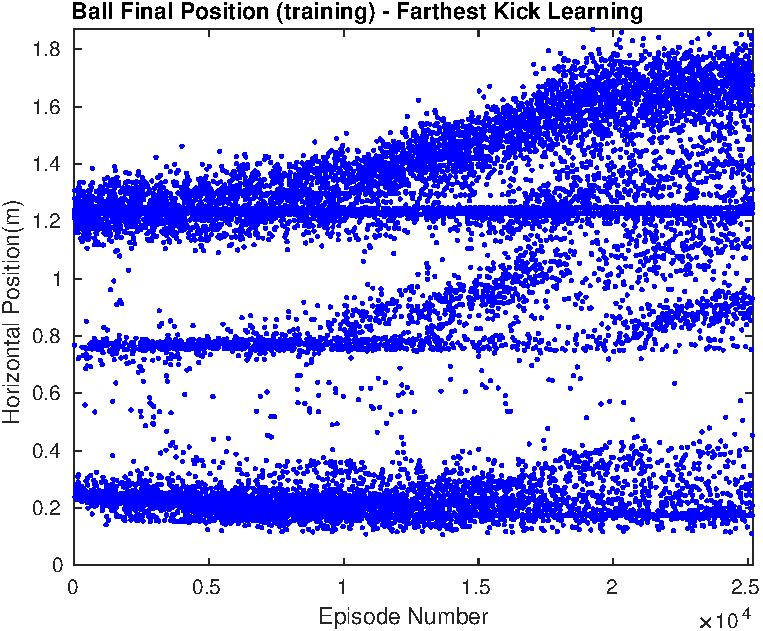
\includegraphics[width=0.6\textwidth]{Chapter7/plots/plot_ball_pos_far_kick_train.pdf} 
    \caption{Ball final positions during training - Farthest Kick task.}
    \label{fig:RL_far_kick_pos_train}
\end{figure}

In the evaluation phase, we turned back to the constant state initialization, starting from a point a few steps after the standard begin of the kick movement, i.e. we ran the ZMP kick during $18.75\%$ of the kick movement, finishing then with the policy.

Also, we turned off the exploration gaussian noise, using solely the mean given by the policy NN. The results follow in Figure \ref{fig:RL_far_kick_pos_eval}, comparing the original final positions from the Pure Mimic trained behavior and the ones achieved by the new Farthest Kick behavior. These statics can also be seen in Table \ref{tab:ppo_far_kick_stat}.

\begin{figure}[H]
    \centering
    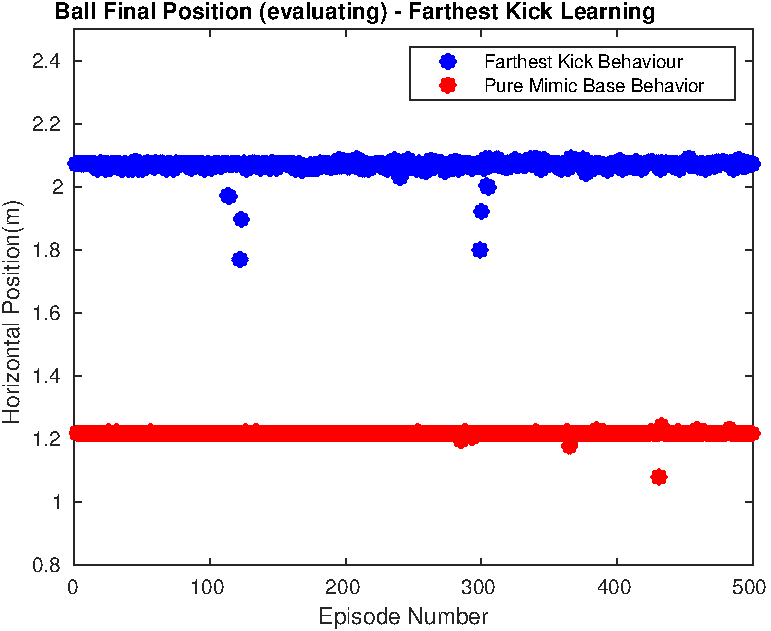
\includegraphics[width=0.6\textwidth]{Chapter7/plots/plot_ball_pos_far_kick_eval.pdf} 
    \caption{Ball final positions during evaluation - Farthest Kick task.}
    \label{fig:RL_far_kick_pos_eval}
\end{figure}

\begin{table}[ht]
    \begin{tabular}{|l|l|l|}
    \hline
      &     Pure Mimic Behavior  &    Farthest Kick Learning  \\ \hline
    Mean             &    $1.2151$  &   $2.0688$    \\
    Std              &    $0.0489$   &  $0.0235$   \\ \hline
    \end{tabular}
\centering
\caption{Farthest Kick Results Statistics}
\label{tab:ppo_far_kick_stat}
\end{table}

In order to illustrate this result in the simulation environment, we show in Figure \ref{fig:RL_far_kick_roboviz} a snap of the game play in RoboViz during the moment the ball reaches its final position. 

\begin{figure}[H]
    \centering
    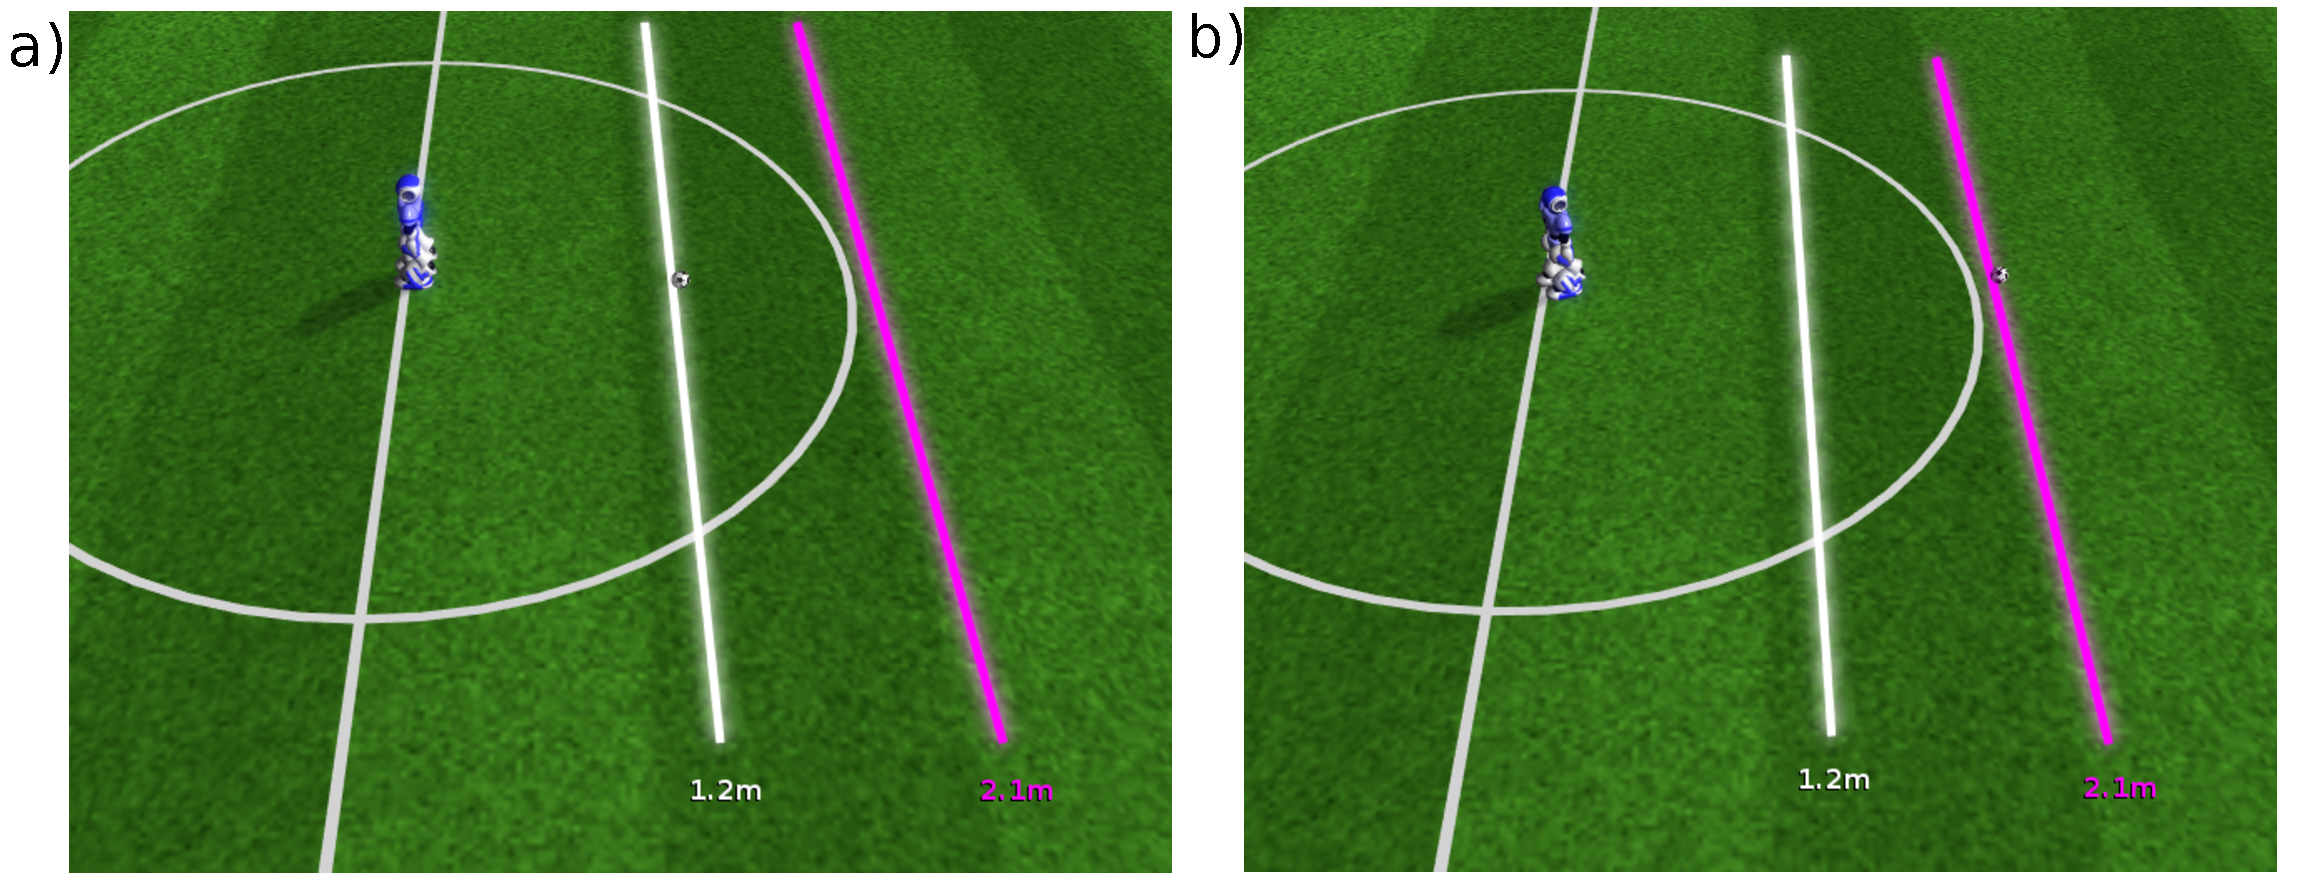
\includegraphics[width=1.0\textwidth]{Chapter7/figures/kick_far.pdf} 
    \caption{Game play illustration. a)Reference final position. b)Learned behavior final position}
    \label{fig:RL_far_kick_roboviz}
\end{figure}

The reward weights described in Section \ref{sec:far_kick_description} we used for this experiment follow in table \ref{tab:weights_far_kick}.

\begin{table}[ht]
    \begin{tabular}{|l|l|}
    \hline
    Hyperparameter            & Value    \\ \hline
    $\omega^p$ 	              & $0.73$ \\
    $\omega^e$                  & $0.16$     \\
    $\omega^c$                & $0.11$     \\
    $\omega^I$					&	$0.3$  	\\
    $\omega^G$					& 	$0.3$		\\
    \hline
    \end{tabular}
\centering
\caption{Reward weights for the Farthest Final Distance task.}
\label{tab:weights_far_kick}
\end{table}

\section{Fixed Final Distance Learning}

In the Fixed Final Distance Learning experiment, we ran PPO with 20 simulated agents using $10^8$ total samples. The hyperparameters are the same used for the Farthest Final Distance task, and follow in Table \ref{tab:fix_kick}.

\begin{table}[ht]
    \begin{tabular}{|l|l|}
    \hline
    Hyperparameter            & Value    \\  \hline
    Adam stepsize             & $10^{-5}$ \\
    Num. epochs               & $10$     \\
    Minibatch size            & $2048$     \\
    GAE parameter ($\lambda$) & $0.95$   \\
    Discount ($\gamma$)       & $0.9999$ \\
    Timesteps per batch       & $4096$   \\ \hline
    \end{tabular}
\centering
\caption{PPO hyperparameters used for Fixed Final Distance Learning.}
\label{tab:fix_kick}
\end{table}

The adaptations made for the Farthest Final Distance task, described in previous Section \ref{sec:far_kick_results}, were essential for this task as well.

We can see that the agent was successful in learning to kick at the final distances of $0.8m$ and $1.5m$, but these results could easily be extended for other fixed positions.

Figures \ref{fig:RL_08_kick} and \ref{fig:RL_15_kick} show the average reward signal during the training phase, presenting some significant increasing.

\begin{figure}[H]
    \centering
    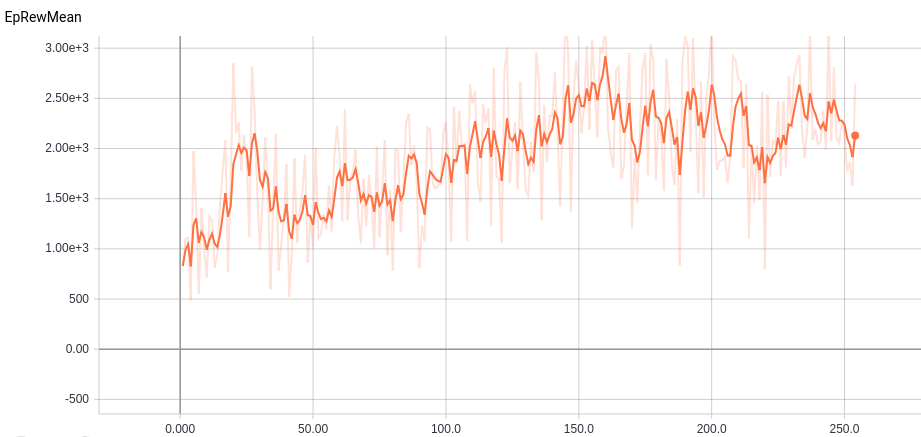
\includegraphics[width=0.8\textwidth]{Chapter7/figures/rew_mean_fix_08.png} 
    \caption{Reward signal during training for the fixed 0.8 distance task.}
    \label{fig:RL_08_kick}
\end{figure}

\begin{figure}[H]
    \centering
    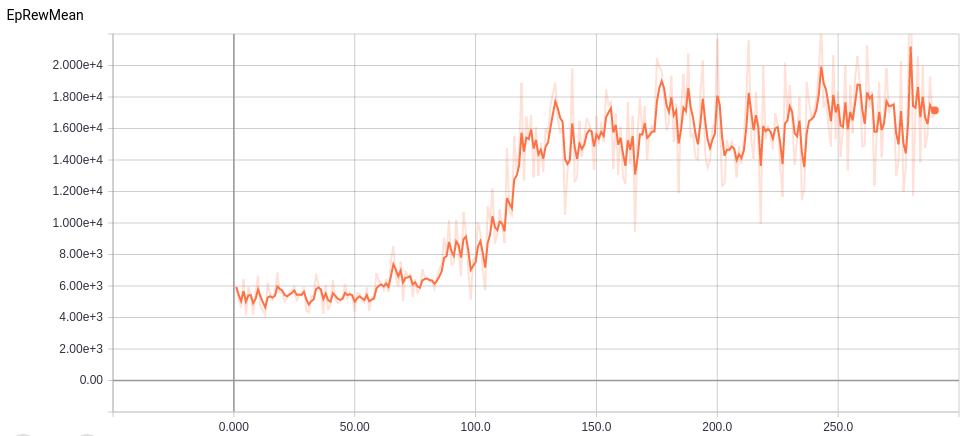
\includegraphics[width=0.8\textwidth]{Chapter7/figures/rew_mean_fix_15.png} 
    \caption{Reward signal during training for the fixed 1.5 distance task.}
    \label{fig:RL_15_kick}
\end{figure}


Figures \ref{fig:RL_08_kick_pos_train} and \ref{fig:RL_15_kick_pos_train} show the final positions for the ball during the training phase, indicating some movement towards the desired position along the training. These distances preserve a high noise though, with a significant fraction of the points still reaching the original distance of $1.2m$. This is mostly caused by the RSI, since it strongly depends on the starting point.

\begin{figure}[H]
    \centering
    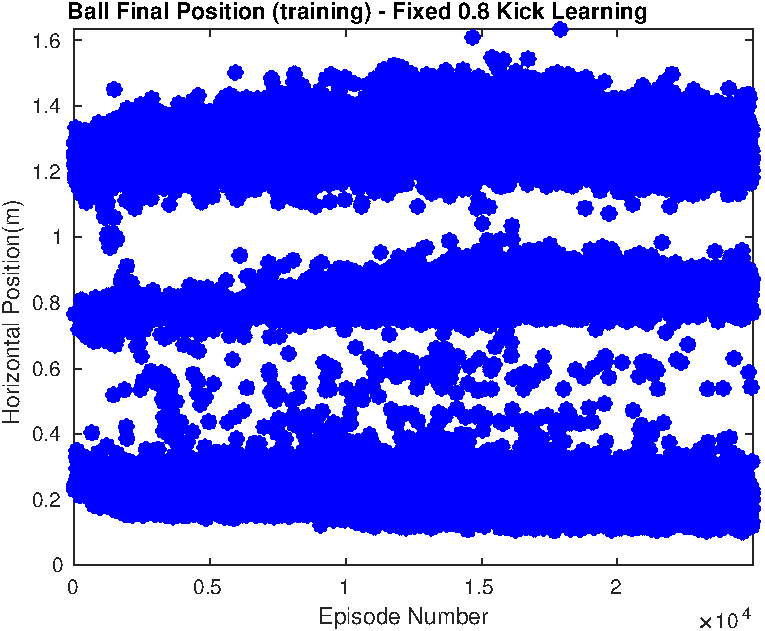
\includegraphics[width=0.6\textwidth]{Chapter7/plots/plot_ball_pos_08fix_kick_train.pdf} 
    \caption{Ball final positions during training - fixed 0.8 distance task.}
    \label{fig:RL_08_kick_pos_train}
\end{figure}

\begin{figure}[H]
    \centering
    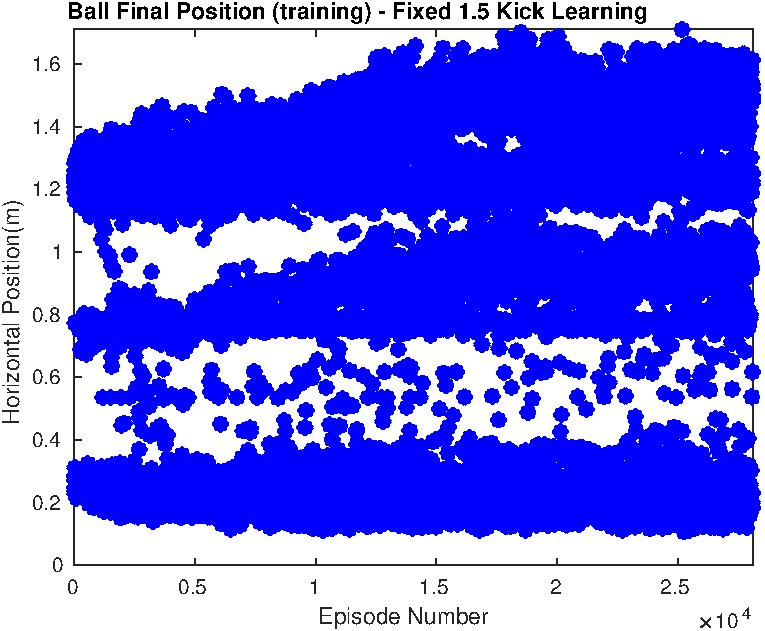
\includegraphics[width=0.6\textwidth]{Chapter7/plots/plot_ball_pos_15fix_kick_train.pdf} 
    \caption{Ball final positions during training - fixed 1.5 distance task.}
    \label{fig:RL_15_kick_pos_train}
\end{figure}

In the evaluation phase, Figures \ref{fig:RL_08_kick_pos_eval} and \ref{fig:RL_15_kick_pos_eval} show the results comparing the obtained behavior with the Pure Mimic Base one. Again, we turned off the exploration noise and initialize at a constant point a few steps ahead of the standard kick begin ($18.75\%$). Moreover, the statistics for these tests can also be seen in Tables \ref{tab:ppo_08_kick_stat} and \ref{tab:ppo_15_kick_stat}.

\begin{figure}[H]
    \centering
    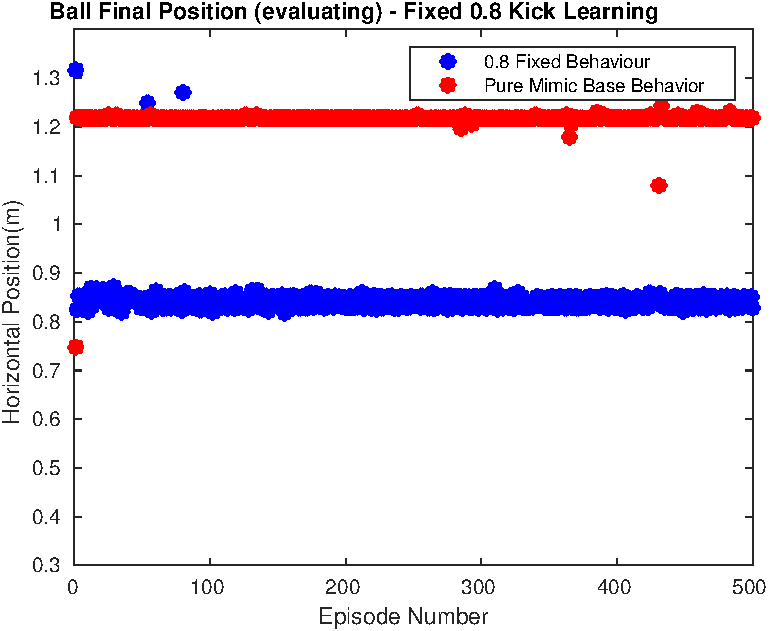
\includegraphics[width=0.6\textwidth]{Chapter7/plots/plot_ball_pos_08fix_kick_eval.pdf} 
    \caption{Ball final positions during evaluation - fixed 0.8 distance task.}
    \label{fig:RL_08_kick_pos_eval}
\end{figure}

\begin{table}[ht]
    \begin{tabular}{|l|l|l|}
    \hline
      &     Pure Mimic Behavior  &    Fixed $0.8m$ kick  \\ \hline
    Mean             &    $1.2151$  &   $0.8434$    \\
    Std              &    $0.0489$   &  $0.0358$   \\ \hline
    \end{tabular}
\centering
\caption{Fixed $0.8m$ Kick Results Statistics}
\label{tab:ppo_08_kick_stat}
\end{table}

\begin{figure}[H]
    \centering
    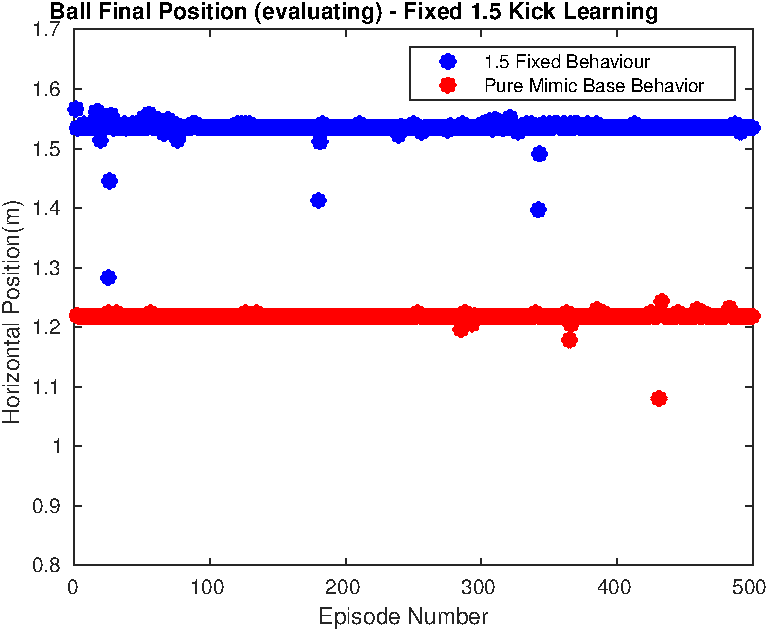
\includegraphics[width=0.6\textwidth]{Chapter7/plots/plot_ball_pos_15fix_kick_eval.pdf} 
    \caption{Ball final positions during evaluation - fixed 1.5 distance task.}
    \label{fig:RL_15_kick_pos_eval}
\end{figure}

\begin{table}[ht]
    \begin{tabular}{|l|l|l|}
    \hline
      &     Pure Mimic Behavior  &    Fixed $1.5m$ kick  \\ \hline
    Mean             &    $1.2151$  &   $1.5349$    \\
    Std              &    $0.0489$   &  $0.0154$   \\ \hline
    \end{tabular}
\centering
\caption{Fixed $1.5m$ Kick Results Statistics}
\label{tab:ppo_15_kick_stat}
\end{table}

Finally, Figures \ref{fig:RL_08_kick_roboviz} and \ref{fig:RL_15_kick_roboviz} present an illustration of these results in the simulation environment using RoboViz. We took a picture of the game play at the instant the ball reaches its final positions.

\begin{figure}[H]
    \centering
    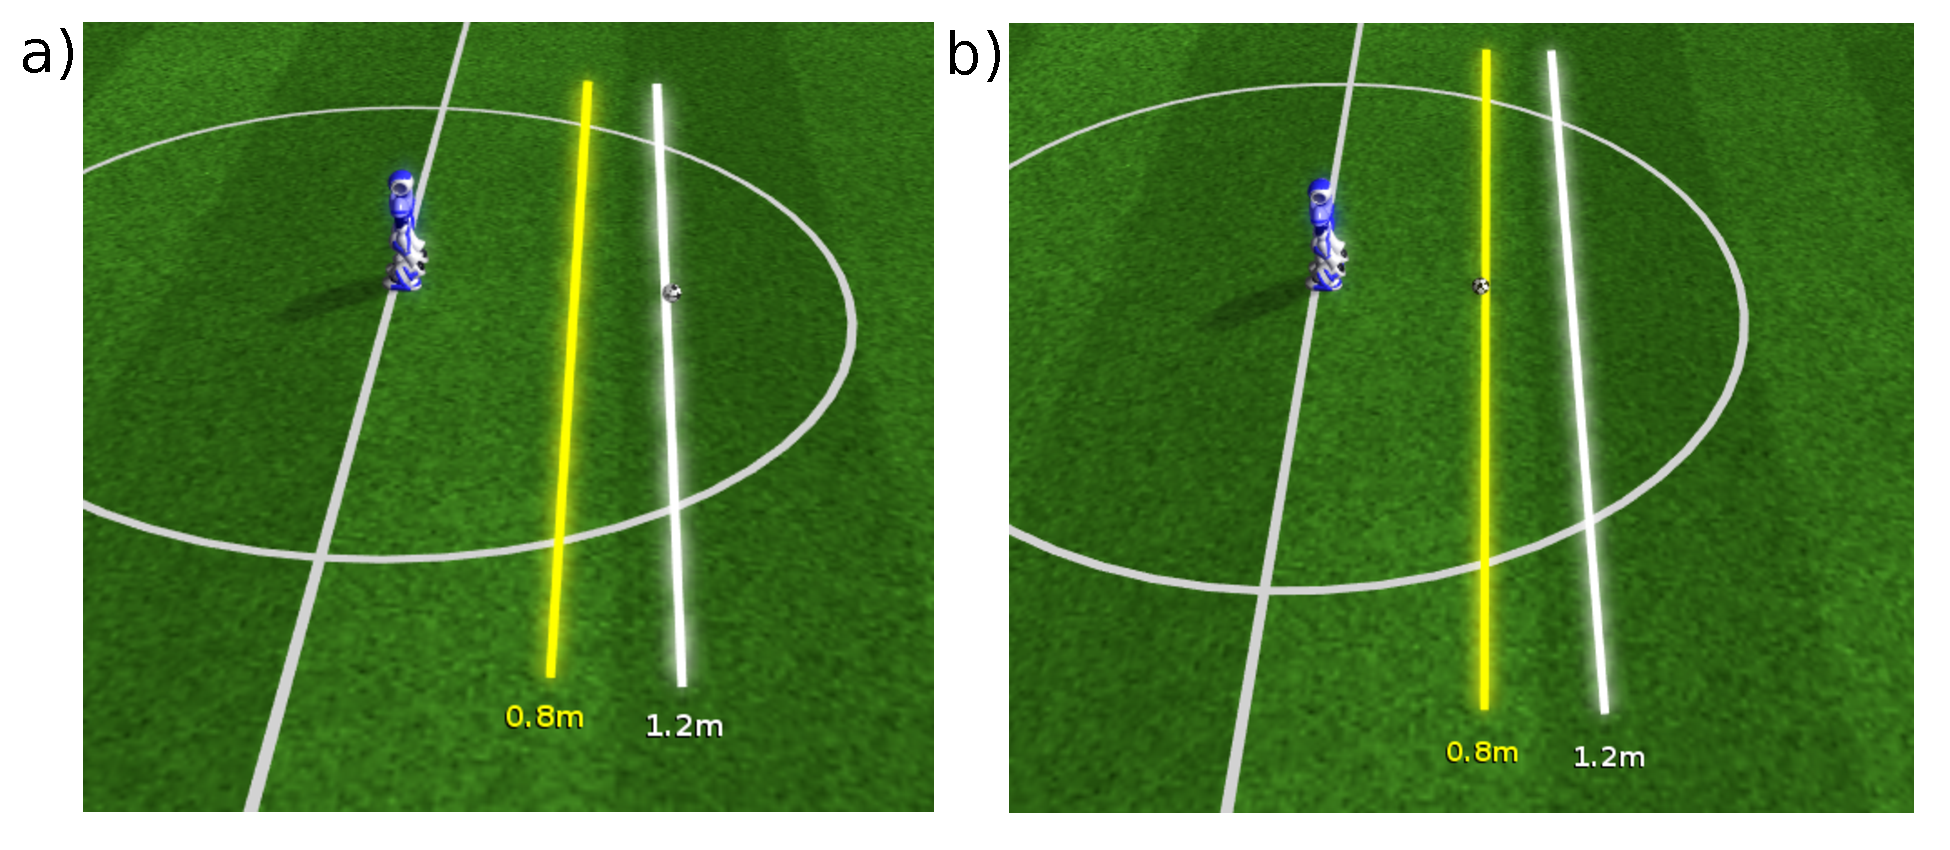
\includegraphics[width=1.0\textwidth]{Chapter7/figures/kick_train_08.pdf} 
    \caption{Game play illustration. a)Reference final position. b)Learned behavior final position}
    \label{fig:RL_08_kick_roboviz}
\end{figure}

\begin{figure}[H]
    \centering
    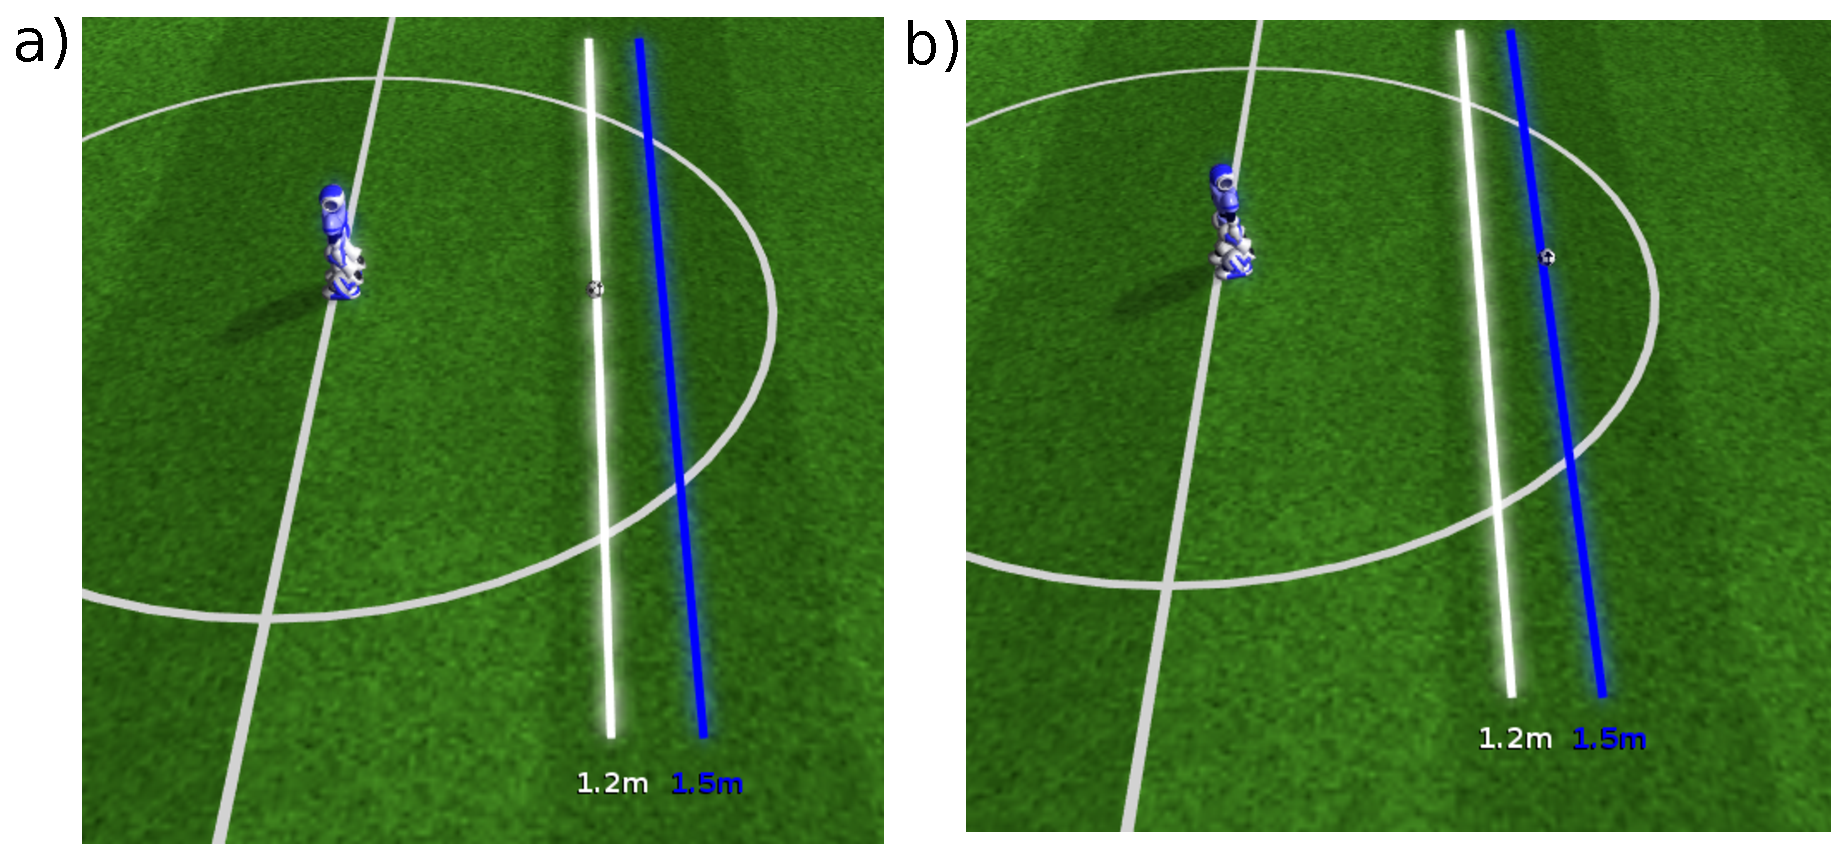
\includegraphics[width=1.0\textwidth]{Chapter7/figures/kick_train_15.pdf} 
    \caption{Game play illustration. a)Reference final position. b)Learned behavior final position}
    \label{fig:RL_15_kick_roboviz}
\end{figure}


%\begin{table}[ht]
%    \begin{tabular}{|l|l|}
%    \hline
%    Hyperparameter            & Value    \\ \hline
%    Adam stepsize             & $3 \times 10^6$ \\
%    Num. epochs               & $10$     \\
%    Minibatch size            & $64$     \\
%    GAE parameter ($\lambda$) & $0.95$   \\
%    Timesteps per batch       & $2048$   \\ \hline
%    \end{tabular}
%\centering
%\caption{PPO hyperparameters used for all three tasks.}
%\label{tab:ppo}
%\end{table}

